
%(BEGIN_QUESTION)
% Copyright 2014, Tony R. Kuphaldt, released under the Creative Commons Attribution License (v 1.0)
% This means you may do almost anything with this work of mine, so long as you give me proper credit

This solvent storage tank is kept heated to 95 degrees F by a steam heat exchanger inside the tank.  Steam is admitted to the exchanger ``loop'' through temperature control valve TCV-105, and exits the loop through a steam trap:

$$\includegraphics[width=15.5cm]{i0006rx01.eps}$$

Suppose one day you notice that pressure gauge PG-361 registers 22 PSI while temperature gauge TG-205 registers 234 degrees F.  Based on this information, determine whether the fluid in that pipe is {\it steam} (vapor) or {\it water} (liquid).  Be sure to explain how you were able to make this determination.

\vfil 

\underbar{file i00043}
\eject
%(END_QUESTION)





%(BEGIN_ANSWER)

This is a graded question -- no answers or hints given!

%(END_ANSWER)





%(BEGIN_NOTES)

The fluid inside this pipe is water, assuming both gauge readings are accurate.  According to a steam table, the saturated steam temperature for water at 22 PSIG (36.7 PSIA) is approximately 262 degrees F.  In other words, it takes a temperature of 262 $^{o}$F to make water boil at a pressure of 22 PSIG.  Since this pipe is colder than 262 $^{o}$F, we know that the pipe must contain (non-boiling) water and no steam.

\vskip 10pt

Another approach is to consult a steam table for the saturated steam pressure at the given temperature of 234 degrees F.  Here, we find the pressure is 22.37 PSIA, which is less than the 22 PSIG (36.7 PSIA) stated in the problem.  This means there is adequate pressure in the system to maintain the water in a non-boiling (i.e. fully liquid) state and therefore there can be no steam.


%INDEX% Physics, heat and temperature: saturated steam pressure versus temperature
%INDEX% Physics, heat and temperature: steam table
%INDEX% Process: solvent storage tank (realistic P&ID shown)

%(END_NOTES)


